\documentclass{standalone}
\usepackage{tikz}
\usepackage{float}
\usepackage{amsmath}
\usepackage{lmodern}
\usepackage{amssymb}
\usetikzlibrary{calc}
\usetikzlibrary{hobby}
\usetikzlibrary{decorations.markings}
\usetikzlibrary{patterns, patterns.meta}
\usetikzlibrary{shapes}
\usepackage{pgfplots}
\tikzset{
    cross/.style={cross out, draw=red, fill=none, minimum size=2*(#1-\pgflinewidth), inner sep=0pt, outer sep=0pt,line width = 0.8pt}, cross/.default={2.8pt},
  % style to apply some styles to each segment of a path
  on each segment/.style={
    decorate,
    decoration={
      show path construction,
      moveto code={},
      lineto code={
        \path [#1]
        (\tikzinputsegmentfirst) -- (\tikzinputsegmentlast);
      },
      curveto code={
        \path [#1] (\tikzinputsegmentfirst)
        .. controls
        (\tikzinputsegmentsupporta) and (\tikzinputsegmentsupportb)
        ..
        (\tikzinputsegmentlast);
      },
      closepath code={
        \path [#1]
        (\tikzinputsegmentfirst) -- (\tikzinputsegmentlast);
      },
    },
  },
  % style to add an arrow in the middle of a path
  mid arrow/.style={postaction={decorate,decoration={
        markings,
        mark=at position .5 with {\arrow[#1]{stealth}}
      }}},
}
\tikzset{arrowstyle/.style={->, >=stealth}}
\pgfplotsset{compat=1.18}
\begin{document}

\centering

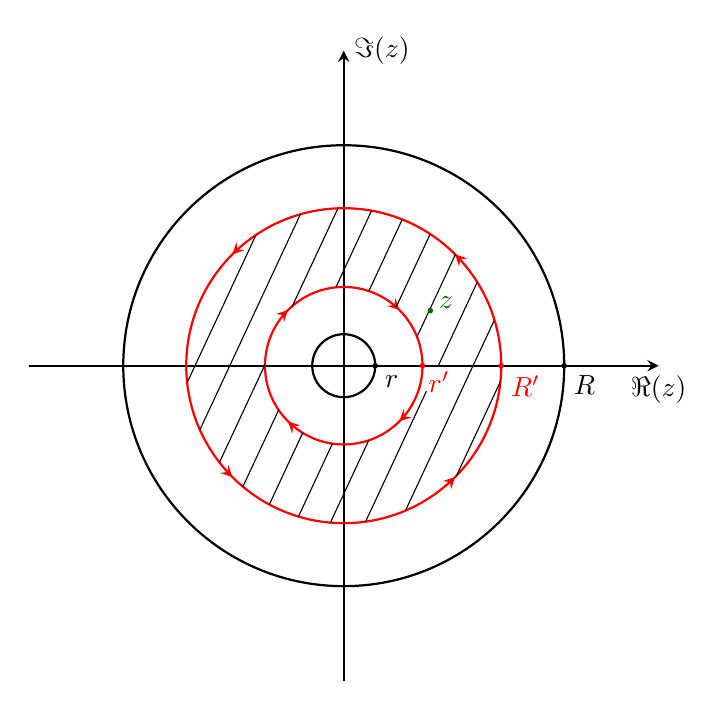
\begin{tikzpicture}
    % draw axes
    \coordinate (O) at (0,0);
    \draw[arrowstyle,thick] (0,-4) -- (0,4) node[anchor=west] {$\Im(z)$};
    \draw[arrowstyle,thick] (-4,0) -- (4,0) node[anchor=north] {$\Re(z)$};

    % Draw circles with radius 1 and 2
    \draw[red, thick,postaction={on each segment={mid arrow=red}}] 
    (1,0) arc[start angle=0, end angle=-360, radius=1];
    \path[draw=red,thick,postaction={on each segment={mid arrow=red}}] (0,0) circle (2);
    
    % draw domain
    \draw[thick](0.4,0) arc[start angle=0, end angle=-360, radius=0.4];
    \draw[thick](2.8,0) arc[start angle=0, end angle=-360, radius=2.8];

    % hatch integration area
    \begin{scope}
        \clip (0,0) circle (2); % Clip at the outer circle
        \fill[even odd rule,pattern={Lines[angle=65, distance=0.4cm]}] (0,0) circle (2) circle (1); % Hatch the outer region
        %\fill[white] (0,0) circle (1); % Exclude the inner circle by filling it with white
    \end{scope}

    % add nodes
    \coordinate (p1) at (0.4,0);
    \coordinate (p2) at (1,0);
    \coordinate (p3) at (2,0);
    \coordinate (p4) at (2.8,0);
    
    \fill (p1) circle (1pt);
    \fill[red] (p2) circle (1pt);
    \fill[red] (p3) circle (1pt);
    \fill (p4) circle (1pt);
    
    \draw (p1) node[below right] {$r$};
    \node at ($(p2) + (6pt, -6pt)$) [draw=white, circle, inner sep=0, fill=white] {\textcolor{red}{$r'$}};
    \draw (p3) node[below right] {\textcolor{red}{$R'$}};
    \draw (p4) node[below right] {$R$};

    % draw z
    \node at (1.3,0.8) [draw=white, circle, inner sep=0, fill=white] {\textcolor{black!60!green}{$z$}};
    \fill[black!60!green] (1.1,0.7) circle (1pt);
\end{tikzpicture}
\end{document}